In the first part of the experiment the rotor’s behavior without external forces was observed, for this the rotor was rotated by hand. After this the base was rotated, during the rotation of the base the rotor remained stationary. This is caused by conservation of angular momentum. Angular momentum conservation also explains why it is only possible to throw a flat object over a long distance if it has spin; a spinning object resists changes in its orientation, this stabilizes the object's flight and keeps it flat, reducing wobbling.
	The gyroscope would only precess if a torque was applied to it, this was done by adding weights to the setup. The weight had a mass of $(29.9 \pm 0.1)*10^-3 kg,$ the masses were placed at distances of $19.9 \pm 0.1 cm$ and $33.2 \pm 0.4 cm$ from the vertical axis of the gyroscope.
	Next the moment of inertia of the rotor around its own axis was determined, this was done using the equation:
\begin{equation*}
    I_3 = \frac{1}{2} M_d R_d^2
\end{equation*}
Where $M_d$ is the mass of the rotor disc, this was given to be $1.74 kg$ and $R_d$ is the radius of the disc, which was $12.47 \pm 0.04 cm$. Substituting in the values of $M_d$ and $R_d$ gave $I_3 = 0.0271 \pm 0.0004 kgm^2$.
    After this $T_3$ was calculated by the following equation:
\begin{equation*}
    T_3 = \frac{10}{Ar}
\end{equation*}
Where $Ar$ is the average rotaions per 10 seconds, which was determined by filming the setup an dividing the film in 10 second long clips, counting the rotations per clip and then taking the average. The differnt values of $T_3$ are shown in Table x in the appendix.
    The previous measured components were used to calculate $T_{p, \text{calculated}}$ using:
\begin{equation*}
    T_{p, \text{calculated}} = \frac{4\pi^2I_3}{MglT_3}
\end{equation*}
$T_{p, \text{measured}}$ was calculated using:
\begin{equation*}
    T_{p, \text{measured}} = \frac{2\pi}{\Omega}
\end{equation*}
$T_{p, \text{calculated}}$ was plotted against $T_{p, \text{measured}}$ in \ref{fig:gyro}.

\begin{figure}[h!]
    \centering
    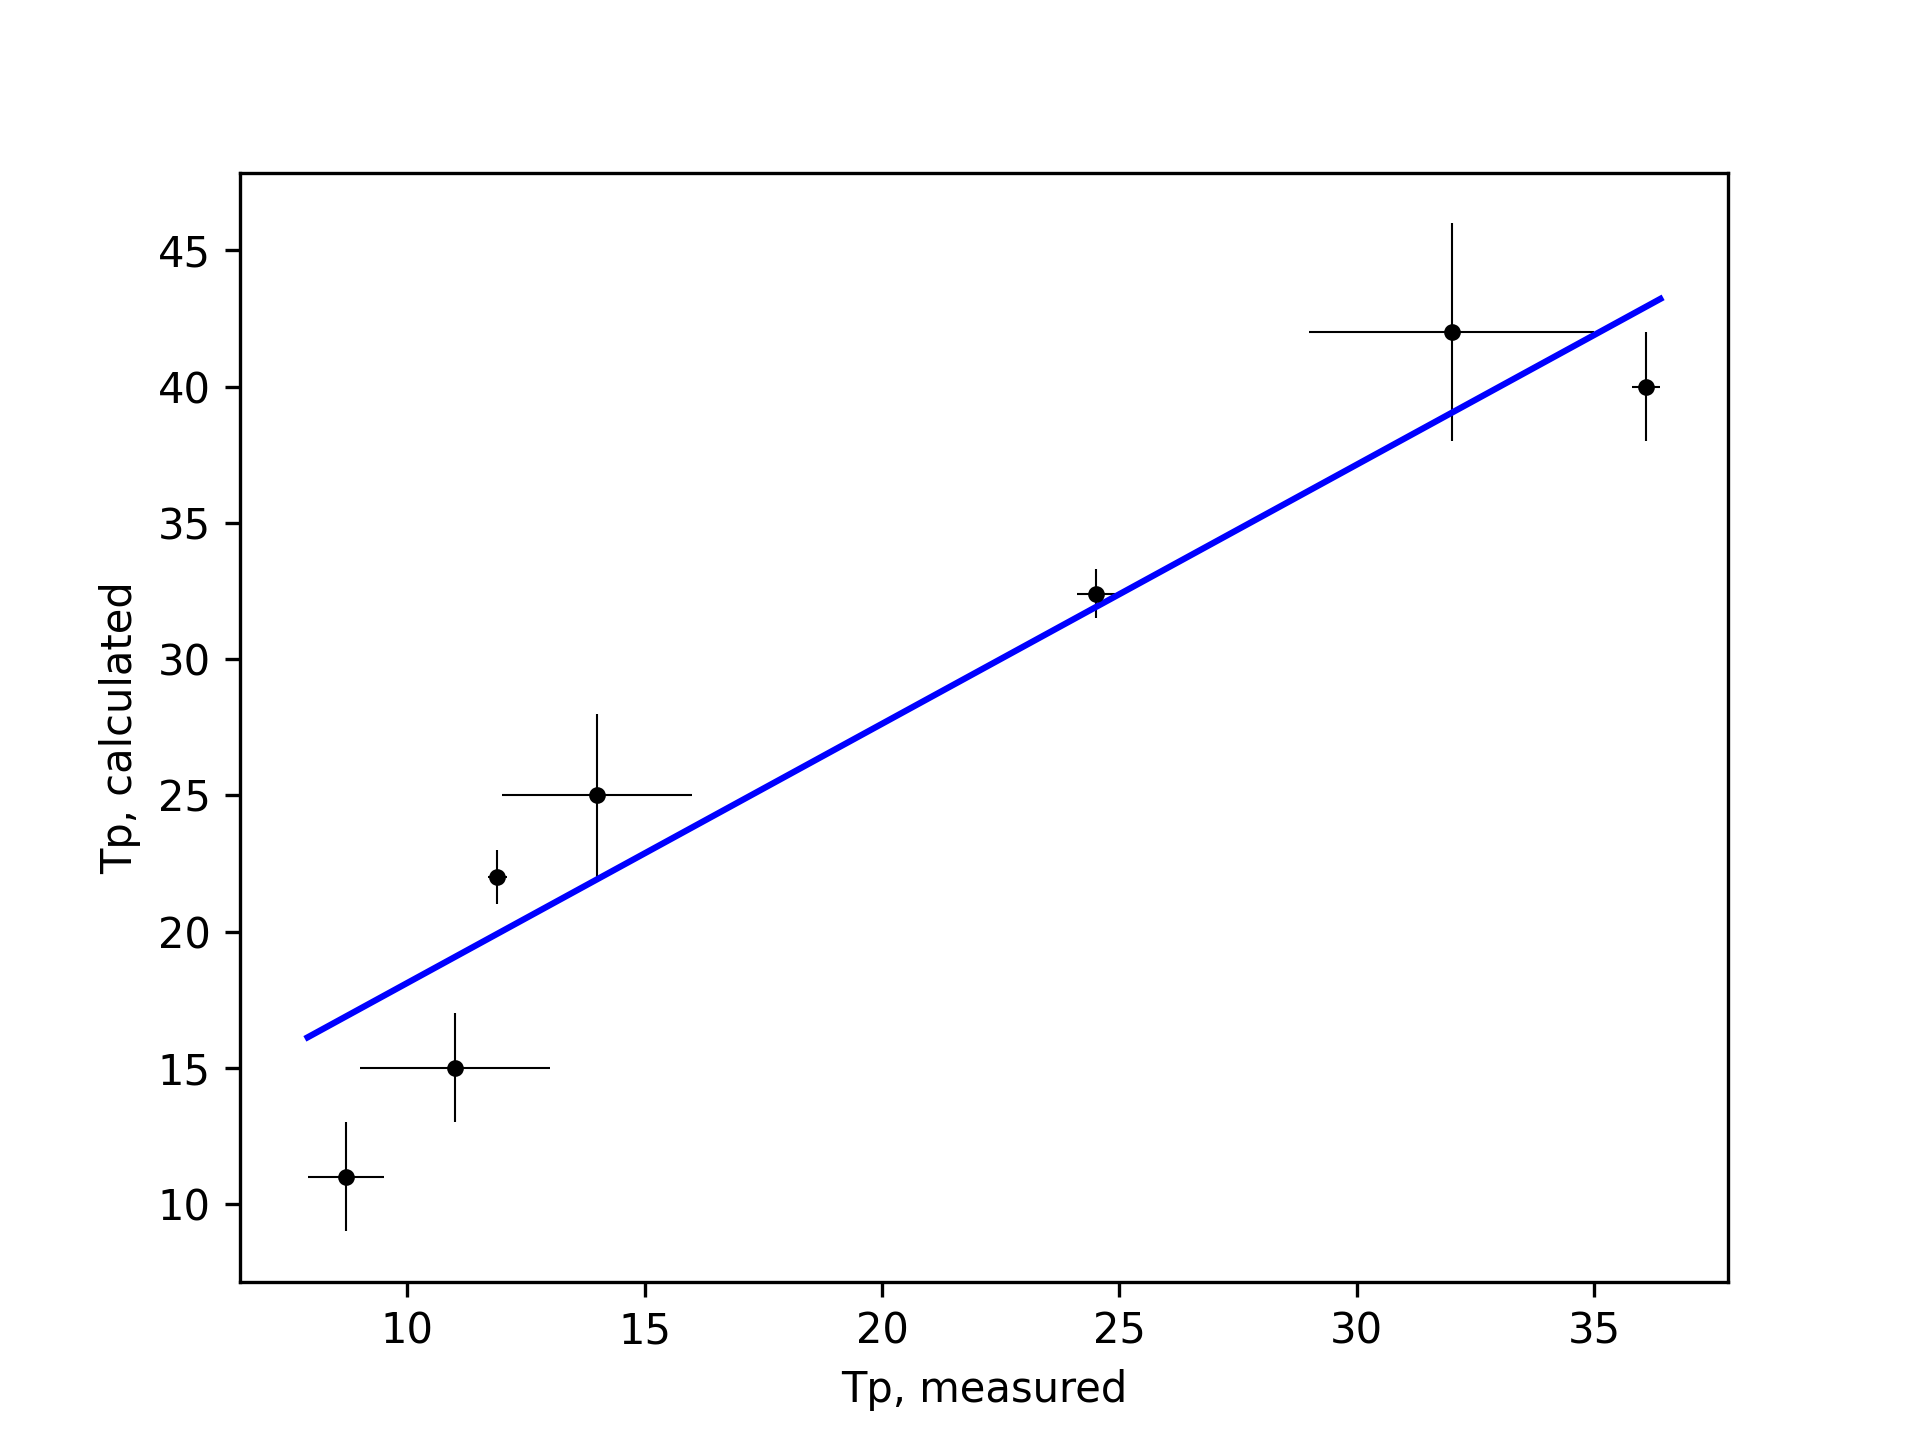
\includegraphics[width=0.8\textwidth]{gyroscope/images/gyro}
    \caption{Correlation between calculated and measured precession periods}
    \label{fig:gyro}
\end{figure}

The line of best fit has a slope of $1.0 \pm 0.2$.